\chapter{Multisignature}
\label{capitolo4}
In this chapter we want to analyse the most important feature of Schnorr Signature: Multisignature.\\
Firstly, we focus on \textit{additivity}, which is the property that leads to the main core of our work.\\
We continue showing the scheme that we have implemented and, finally, we analyse the reasons behind every choice taken.\\

\section{Key Aggregation}
The biggest innovation brought by Schnorr signature is the \textit{Key Aggregation}, which, according to \cite{MuSig}, means that the joint signature can be verified exactly as a standard Schnorr signature with respect to a single "aggregated" public key which can be computed from the individual public keys of the signers.\\
Key aggregation is closely related to \textit{additivity}.
\subsection{Additivity}
\textit{Additivity} is a very important property of Schnorr signature.
In \cite{NovAdd}, Greg Friedman introduces the connection between additivity and additive signature:\\
given two manifolds $M_{1}$, $M_{2}$ glued together along a common boundary. \textit{Additivity} holds when the signature is additive with respect to this decomposition.\\
In order to understand this statement, Friedman introduces bilinear forms. In particular, given a bilinear form on finite dimensional $\mathbb{R}$-vector spaces
\begin{equation*}
\phi:V \otimes V \to \mathbb{R},
\end{equation*}

it is symmetric if $\phi(v,u)=\phi(u,v)$ $\forall v,u \in V$. The matrix representation is $M_{ij}=\phi (e_{i},e_{j})$.\\
Two of the considerations he does in the paper, are very important for our implementation:
\begin{quote}
	\begin{itemize}
		\item $(V_{1},\phi_{1}),\ (V_{2},\phi_{2})$ produces $\phi_{1} \boxplus \phi_{2}$ on $ V_{1}\oplus V_{2}$:
		\[ 
		\begin{pmatrix}
			 \phi _{1}  & 0\\
			0 &  \phi_{2} 
		\end{pmatrix} 
		\]
		The signature of the sum is the sum of the signatures.
		\item On $V_{1} \bigotimes V_{2}$, there is a natural form. The signature $\sigma(\phi_{1}\otimes \phi_{2})= \sigma(\phi_{1}) \sigma(\phi_{2})$
	\end{itemize}
\end{quote}

Both the considerations have an important implication:\\
since the elliptic curve is a finite dimensional $\mathbb{R}$-vector space, Schnorr signature is additive.\\
We have taken advantage of this property and we have implemented a \textit{multisignature} scheme.

\section{Scheme}
This scheme consists of 3 stages and one preparatory step (Stage 0).
\paragraph{Stage 0} 
Given the elliptic curve domain parameters \textit{(p, a, b, G, n, h)} and The message $m$ to be signed, each user $i$ has to generate his key pair $(p_{i},P_{i})$.\\

\textbf{Inputs:} Every signer $i$ has to provide his public key $P_{i}$.

\textbf{Actions:} The following actions are performed:

\hspace{1.2cm}
\begin{minipage}[l]{2\linewidth}
	\begin{enumerate}
		\item The hash value of $P_{i}$, $h_{i}=H(P_{i})$.
		\item $P_{All}=\sum_{i} h_{i}\times P_{i}.$
	\end{enumerate}
\end{minipage}

\textbf{Output:} $P_{All}$.

\paragraph{Stage 1}

Every signer $i$ has to choose his ephemeral nonce $k_{i}$, compute the \textit{Ephemeral key} $K_{i}$ and give to the other signers the $x$ coordinate $K_{x_{i}}$

\paragraph{Stage 2}
In this stage everyone computes his own signature $s_{i}$ and the \textit{Ephemeral key} related to the \textit{multisignature}. Everyone has to follow this process.\\
\textbf{Inputs:} Every signer $i$ has the following informations as inputs.

\hspace{1.1cm}
\begin{minipage}[l]{2\linewidth}
	\begin{enumerate}
		\item The message $m$.
		\item His private key $p_{i}$.
		\item His \textit{ephemeral key pair} ($k_{i}, K_{i}$).
		\item The $x$ coordinate of the \textit{ephemeral key} of the other signers, $K_{x_{j}},\ \forall j\neq i$
	\end{enumerate}
\end{minipage}


\textbf{Actions:} Every user, indipendently from the others, performs the following instructions:

\hspace{1.2cm}
\begin{minipage}[l]{2\linewidth}
	\begin{enumerate}
		\item $p_{i}= p_{i}\times h_{i}$
		\item if $K_{i}$ is odd:
		\begin{itemize}
			\item[a.] $k_{i}=n-k_{i}$
			\item[b.] $K_{y_{i}}=p-K_{y_{i}}$
		\end{itemize}
		\item $\forall j\neq i$, $i$ recovers $K_{j}$
		\item $K_{All_{i}}=\sum_{j\neq i}\ {K_{j}}+K_{i}$
		\item if $K_{All_{i}}$ is odd:
		\begin{itemize}
			\item[a.] $k_{i}=n-k_{i}$
			\item[b.] $K_{All_{y_{i}}}=p-K_{All_{y_{i}}}$
		\end{itemize}
		\item $h_{i}=H(m||K_{All_{i_{x}}})$\\
		If $h_{i}=0$ \ mod\ $n$ goto 1.
		\item $s_{i}=k_{i} - h_{i} \times p_{i} \bmod\ n$ \\
		If $s_{i}=0$ goto 1.
	\end{enumerate}
\end{minipage}

\textbf{Output:} $(K_{All_{x_{i}}}, s_{i})$
\paragraph{Stage 3}
In this stage, takes place the combination of the previous outputs, in order to compute the final signature.\\
\textbf{Inputs:} Every signer $i$ has to provide the following informations as inputs.

\hspace{1.1cm}
\begin{minipage}[l]{2\linewidth}
	\begin{enumerate}
		\item $K_{All_{x_{i}}}$.
		\item His signature $s_{i}$.\\
	\end{enumerate}
\end{minipage}


\textbf{Actions:} The following instructions are performed:

\hspace{1.2cm}
\begin{minipage}[l]{2\linewidth}
	\begin{enumerate}
		\item if $K_{All_{x_{i}}}=K_{All_{x_{j}}}$ $\forall i,j$: $K_{All_{x}}= K_{All_{x_{i}}}$.
		\item else: fail.
		\item $s_{All}=\sum_{i}{s_{i}}$.
		If $s_{All}=0$ or $s_{All}\geq order$: fail.
	\end{enumerate}
\end{minipage}

\textbf{Output:} The Multisignature $(K_{All_{x}}, s_{All})$ over $m$

We want to highlight that along the process the signers have to communicate each other some informations, such as between stage 1 and 2: among the inputs of stage 2 there are the $x$ coordinate of the \textit{ephemeral key} of the other cosigners.
\subsection{Verification}
Through the process explained above, we have obtained one signature in place of $N$ single signatures. The most fascinating property is that this signature acts as a single one, so the verification process is the same presented in Chapter \eqref{capitolo3}, but in this case the inputs are slightly different: $P_{All}$ in place of the single $P_{i}$.


\section{Step by step analysis}
Now we want to highlight the purpose of each step delineated above.\\
We should start with stage 1, where signers have to communicate the $x$ coordinate of their \textit{Ephemeral key}, $K_{x}$. This step is fundamental because in stage 2 everyone has to recover the \textit{ephemeral} keys of the cosigners in order to compute $K_{All_{i}}$. Otherwise it would not be possible to generate a key aggregation using the additivity property. Actually, the users could send their entire $K_{i}$, but it would duplicate the cost of communication obtaining the same result. Not by chance, we ask to controll the parity of their own key before sending it: in this way we know that every key is positive.\\
Going on in the second stage, the signatures are generated following the usual scheme.\\
The last steps we should focus on are:
\begin{enumerate}
	\item $P_{All}=\sum_{i} h_{i}\times P_{i}$
	\item $p_{i}=p_{i}\times h_{i}$,
\end{enumerate}
where $h_{i}=H(P_{i})$.\\
In the original idea there were not the $h_{i}$, but they are fundamental. Without them the \textit{Rogue key attack} would be possible.
\subsection{Cancellation attack}
The \textit{Rogue Key attack}, also known as \textit{Cancellation attack}, is an attack made by malicious users who manipulate public keys in order to produce forgeries of the set of public keys.\\
Since everyone knows the various public keys $P_{i}$ and $P_{All}=\sum_{i} P_{i}$, the corrupted signers can easly compute their $P_{i}$ as a combination of all the public keys so that $P_{All}=\sum_{j} P_{j}$ where $j$ are the malicious signers.
\begin{example}
	Let Alice and Bob want to sign the same message $m$ through the \textit{multisignature} scheme where $P_{All}=\sum_{i} P_{i}$.\\
	Alice is honest, while Bob wants to have the controll of the signature all alone.\\
	Bob can compute $P'_{B}=P_{B}-P_{A}$, because $P_{A}$ is known. \\
	$\implies P_{All}=P'_{B}+P_{A}=P_{B}-P_{A}+P_{A}=P_{B}$\\
	The signature is valid and the verifiers are not able to demonstrate that Bob has ripped off Alice and $P'_{B}$ is not his real public key.
\end{example}
This type of attacks was the reason why the first proposals failed and were abandoned. The first solution to this problem came from Micali, Ohta, and Reyzin in 2001, but it was based on an interactive key generation protocol.\\
Another way to prevent Rogue-key attacks is to require the proof of knowledge of the secret key during public key registration, idea proposed by Thomas Ristenpart and Scott Yilek in their paper published in 2007.\\
Both the solutions were highly expensive. We implemented the idea explained in \cite{MuSig}, because it does not require additional interactions between the signers, much more cheaper than the previouse ideas.
\section{Benefits}
We have analyzed \textit{multisignature} in every step, but why have we implemented it?\\
This scheme allows us to save a lot of space, because in place of $n$ signatures we end up with only one!\\
This is fundamental, for example, in Bitcoin system. Bitcoin \cite{Nakamoto} is a digital currency scheme in which all participants (are able to) validate transactions. These transactions consist of outputs, which have a verification key and amount, and inputs which are references to outputs of earlier transactions not spent yet (known as UTXOs). Each input contains a signature. In fact, some outputs even require multiple signatures to be spent. Transactions spending such an output are often referred to as $m$-of-$n$ multisignature transactions, and the current implementation corresponds to the concatenation of the individual signatures. For each transaction are required from one to $m$ signatures. These transactions are stored in a distributed ledger, known as blockchain, composed by connected blocks where the transactions are stuffed into.\\
It is obvious that through a \textit{multisignature} scheme, the signature sizes would be lowered to the standard single signature of 64 bytes, regardless of the number of cosigners. Consequently, the transaction's size would diminish lowering the blocks' weight.\\
In the figure below it is represented the actual blockchain size and the one that it would have had if there had been a multisignature scheme since 2008.
\begin{figure}[H]
	\centering
	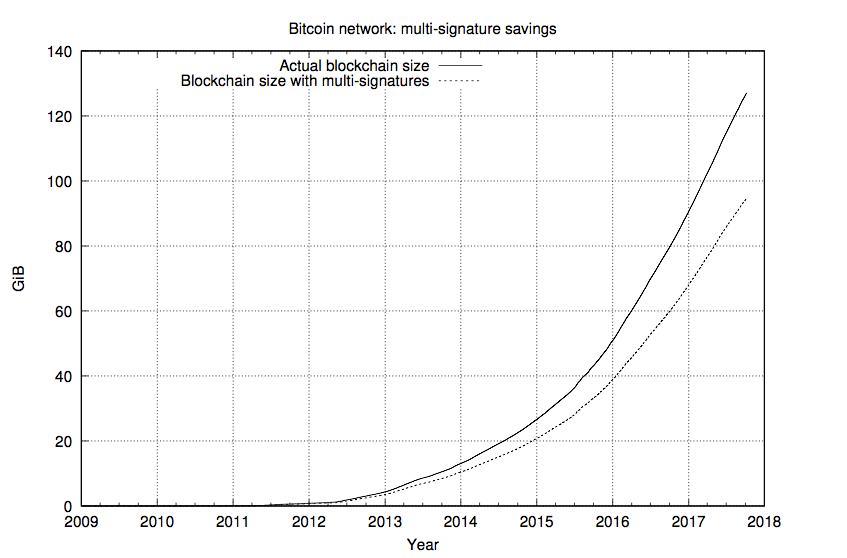
\includegraphics[width=.85\textwidth]{BlockchainMusig.png}
	\caption{Size of the Bitcoin blockchain with and without multi-signatures.}
	\label{img:BlockchainMusig}
\end{figure}